\chapter{Deterministic multitasking}{``No battle plan ever survives contact with the
  enemy.''}{Field Marshall Helmuth Carl Bernard von Moltke}
\label{chap:adv_code}

This chapter presents certain advanced aspects of code generation from
AADL models to Ada source. The major technique introduced in this
chapter is that of deterministic communication connectors between
tasks. This deterministic communication is necessary for the correct
construction of control systems. The other aspect presented is a study
of how to implement mode-specific temporal characteristics of tasks.

\section{Deterministic communication}
Vehicle control systems are one of the most safety-critical categories
of software even within the real-time systems domain. Stringent
standards of code review---such as DO-178B for avionics
systems~\cite{do178b}---must be met before deployment onboard the
platform. Such control systems are invariably implemented in the form
of control laws that take input data from sensors, carry out
transformations on that data and apply the outputs to actuators, as
shown in Fig.~\ref{fig:ctrl_loop}. These control law computations are
always carried out periodically, at a sufficiently high frequency to
keep the concerned platform stable. This is why in literature such
control law implementations are also called ``control loops''. Two
orthogonal sets of requirements are always leveraged on such systems:

\begin{itemize}
\item{Timing requirements relating to the timeliness of the results
  produced, as the validity of results is strongly dependent upon the
  time at which they are available;}
\item{Functional requirements describing the output of the system as a
  function of the input, i.e., the algorithmic portion of the control
  law's response loop.}
\end{itemize}

One of the properties that these systems must exhibit is determinism,
to with that two equivalent runs with the same inputs should produce
the same results. In a process-based executive, data flow between two
threads operating at different periods may cause non-determinism since
their order of execution may change from one run to the next due to
decisions taken by the scheduler. These different orders of execution
may result from, among other things, sporadic threads being dispatched
due to external stimuli.

One approach to achieving this determinism is to use a synchronous
reactive language such as Lustre and its associated SCADE
Suite~\cite{halbwachs@ieee91} or Matlab \simu~\cite{simulink} to
implement the control laws. In this paradigm there is only one thread
of execution and the entire functionality of the control system is
collapsed into it. The various \emph{functional nodes} of the model
are then executed in synchronous lockstep, this ensures a completely
deterministic execution of the various functions of the control
loop. An offline data dependency graph can be constructed using the
data flow information present in the model, this dependency graph
allows the \emph{\`a priori} calculation of the invocation order for
the various functions. In Chapter~\ref{chap:biblio}, examples of both
Lustre and Simulink were provided.

Another approach is to write multi-threaded control applications,
which run atop an operating system with a process based
scheduler~\cite{butler@spie93}. This scheduler will inevitably preempt
and resume the various threads at multiple, arbitrary points. Said
preemptions will introduce a certain amount of non-determinism in the
order of execution. The advantages of this approach are the
possibility of higher processor utilization as well as flexibility of
adding threads later in the design stage. It also allows designers to
\emph{piggyback} non-control threads such as alarm and status monitors
onto the same partition.

In all control systems, communication is carried out in the form of
data flows as this is the paradigm most native to control law
concepts. The system architecture is usually represented in a block
structured formalism where the blocks represent transformations on
data and the lines connecting them the inputs and outputs for those
data transformations. Such an architecture is shown in
Fig.~\ref{fig:ctrl_loop}. The blackbox above computes the
\emph{transfer function}. In a process based---or
asynchronous---control system implementation this would be refined to
a set of periodic threads that exchange data among themselves to
compute the final value of the output, as shown in the callout
balloon.

\begin{figure}
\centering
\includegraphics[scale=1.4]{figs/impulse}
\caption{Control loop and its block diagram}
\label{fig:ctrl_loop}
\end{figure}

The simplest method of implementing a data flow between two co-located
threads in a process-based executive is to use a shared variable
protected against concurrent access by a mutex. However, this
introduces the danger of non-determinism in the data flow, due
normally to auxiliary load on the system. Consider two periodic
threads in a system (\ts and \tl) with periods \pshort and \plong
respectively such that \plong$=3\times$\pshort. In case of the Rate
Monotonic priority assignment and associated runtime using a Fixed
Priority Preemptive Scheduler, the priority of \ts is higher than that
of \tl. Thus, the single job of \tl in each mutual hyperperiod is
executed between jobs of \ts (the mutual hyperperiod of two threads is
defined to be the LCM of their periods). If \ts produces data $\alpha$
to be consumed by \tl then the non-determinism shown in
Fig.~\ref{fig:non_determinism} might result: in the first hyperperiod,
\tl is launched just after \ts finishes its first job and writes
$\alpha_1$, this is read by \tl as the value of the data flow. In the
next hyperperiod, due to extraneous factors---such as a sporadic alarm
thread firing---\tl is executed after the \emph{second} job of \ts and
it reads $\alpha_5$ instead of the expected $\alpha_4$.

Vice-versa, if \tl produces data $\beta$ to be read by \ts then the
following non-determinism might occur (also shown in
Figure~\ref{fig:non_determinism}): in the first hyperperiod, \tl
finishes \emph{after} the last job of \ts and thus all three jobs of
\ts in this hyperperiod use $\beta_0$. However, in the next
hyperperiod, \tl finishes just before the last job of \ts and that job
reads $\beta_2$ instead of $\beta_1$.

This type of non-determinism is unacceptable in control
applications. To guard against this breach, the protocol given in
Fig.~\ref{fig:determinism}---which sacrifices freshness of data for
determinism ---is widely used in control system development. All data
flow values are taken from the last job of the previous mutual
hyperperiod of both threads involved. This eliminates non-determinism
due to scheduling decisions by the RTOS. Even though control laws and
their implementation control loops---due to their repetitive
nature---are resilient to a few discrepant data flows, it is always
preferable have an implementation that is faithful to the law's
formulation. This deterministic data flow will enable a more robust
control law implementation that keeps the platform more stable.

In a purely synchronous system such as that generated by Lustre,
creating such data flow constructs is very simple. Lustre nodes at
different rates (or periods) can be constructed via the use of
conditional invocation of nodes using counters and the \kw{when}
keyword. Previous data from source nodes that are slower than the node
in question can be accessed via judicious use of the \kw{pre} and
\kw{current} keywords. An example of a Lustre system to implement the
data flow $\beta$ from a slow node to a fast node is given in
Listing~\ref{lst:lustre_dataflow}. Two nodes are defined,
\texttt{Fast} and \texttt{Slow}. The driver node \texttt{Main}
instantiates a boolean flow \texttt{C} that is used to invoke the node
\texttt{Slow} once every two steps. The node \texttt{Fast} is invoked
at every step, and it calculates its output \texttt{cmd1} from the
flow \texttt{beta} via the \kw{pre} and \kw{current} keywords to
sample from the previous value calculated by node \texttt{Slow}.

\begin{minipage}{\listingwidth}
\begin{center}
\begin{lstlisting}[language=lustre, label=lst:lustre_dataflow,
    caption=A slow to fast node deterministic data flow in Lustre]
node Fast (beta : int) returns (cmd1 : int)
let
  cmd1 = 0->current(pre(beta))+2;
tel.

node Slow (arg : int) returns (dat : int)
let
  dat = if arg > 0 then arg else (0-arg);
tel.  

-- Driver --
node Main (sensor : int) returns (actuator : int)
var arg : int;
var C   : bool;
let
  -- Create a flow C that alternates between true and false --
  C = true->not pre(C);

  actuator = Fast(beta);
  beta = 0->Slow(arg) when C;
tel.
\end{lstlisting}
\end{center}
\end{minipage}

The same functionality is available in \simu as ``rate transition''
blocks. These blocks should be used in a multi-rate multi-tasking
Simulink model. These blocks need to be placed between other
functional blocks which communicate with each other and which have
different ``rates''. The rate transition blocks ensure data protection
(concurrency safety) as well as determinism in the data flow between
the two blocks they are connected to. An example of the utilisation of
rate transfer blocks is given in Fig.~\ref{fig:rate_transition}. The
block \texttt{Product} runs at twice the rate of \texttt{Product1},
the data flow between them is ensured to be safe and deterministic due
to the \texttt{Rate Transition} block present.

\begin{figure}
\centering
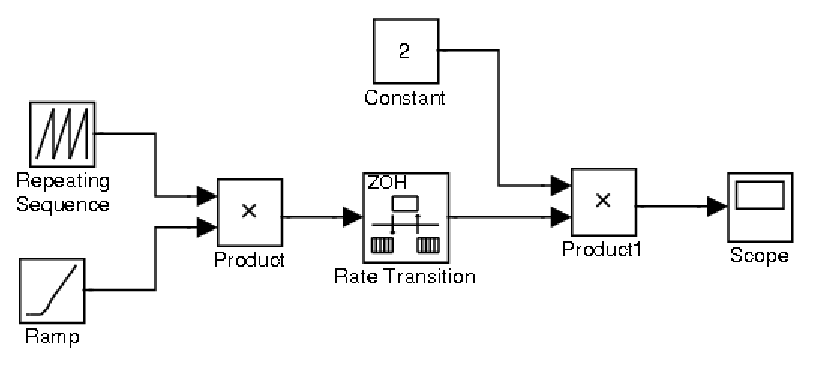
\includegraphics[scale=0.8]{figs/rate_transition}
\caption{Rate transition block between two blocks at different rates
  in Simulink}
\label{fig:rate_transition}
\end{figure}

A similar method for ensuring determinism in data flow is presented in
this section. The basis for the approach used, i.e., special buffering
techniques for shared data buffers, was first presented
in~\cite{tripakis@emsoft05}. This approach, and an extension of it has
been integrated into the modeling notation for AADL, as well as into
the ARC code generator for automatic code generation. This allows the
creation of asynchronous---i.e., process based---real-time control
systems that can incorporate true sporadic threads.

\begin{figure}
\centering
\includegraphics[scale=1.75]{figs/det_breach1}
\caption{Non-determinism in data-flow}
\label{fig:non_determinism}
\end{figure}

\begin{figure}
\centering
\includegraphics[scale=1.75]{figs/det_no_breach}
\caption{Protocol to ensure determinism}
\label{fig:determinism}
\end{figure}

\subsection{Deterministic protocol and its properties}
\label{sec:approach}
This section presents a simple mathematical formulation of the data
flow. However, first an explicit statement of hypotheses that can be
made upon the system needs to be enunciated. These hypotheses are
quite natural and evident for a large class of real-time operating
systems, and are true for a Ravenscar-compliant executive:

\begin{itemize}
\item{The system is hard real-time. Periodic tasks are guaranteed to
  be dispatched at the start of each period (dispatching means being
  put in the ready state, not necessarily being given the processor);}
\item{The release of tasks themselves is synchronous, i.e.: two
  periodic tasks with coincidental release times are dispatched
  concurrently (even though the higher priority task will execute
  first);}
\item{Deadlines are met, otherwise schedulability has been breached
  and the system should go into a graceful degrade mode;}
\item{Both the source and destination threads are periodic with
  \plong=$r\times$\pshort and $r>1$. $r=0$ is a degenerate case and
  if $r=1$ then there is no problem since there will be one job of
  each task in each mutual hyperperiod and the higher priority task
  will always be dispatched first;}
\item{The source thread writes to the data flow and the destination
  thread reads from the data flow at each job;}
\item{The scheduler is preemptive and priority based;}
\item{Priority assignment is rate monotonic~\cite{liu@jacm73}, i.e.,
  \ts has higher priority than \tl. Thus, at the start of each mutual
  hyperperiod \plong, \ts will be \emph{executed} before \tl, even
  though both were made ready simultaneously.}
\end{itemize}

Given the above assumptions a simple mathematical model for the
deterministic data flow can be obtained. For a data flow from a
high-frequency to low-frequency thread every $r^{th}$ write is
used. Similarly, for a data flow from a low-frequency to
high-frequency thread every write is read $r$ times. Let
\tl$(i)\gets\alpha_j$ signify that the $i^{th}$ job of thread \tl gets
the $j^{th}$ instance of data-flow $\alpha$. For the example of
Fig.~\ref{fig:determinism} (\plong$=3\times$\pshort), the first few
data flows are:

\begin{displaymath}
  \begin{split}
  \tau_s(1)\gets\beta_0,\ \tau_s(2)\gets\beta_0,\
  \tau_s(3)\gets\beta_0,\ \tau_s(4)\gets\beta_1\\
  \tau_l(1)\gets\alpha_0,\ \tau_l(2)\gets\alpha_3,\
  \tau_l(3)\gets\alpha_6,\ \tau_l(4)\gets\alpha_9
  \end{split}
\end{displaymath}

\begin{comment}
\begin{equation}\label{eqn:diff_generic}
  \begin{split}
  \forall i\in\mathbb{N}:\tau_s(3i+1)\gets\beta_i,\
  &\tau_s(3i+2)\gets\beta_i,\ \tau_s(3i+3)\gets\beta_i\\
  \forall i&:\tau_l(i)\gets\alpha_3(i-1)
\end{split}
\end{equation}
\end{comment}

These equations can be formulated for the general case as well,
assuming that the ratio between \plong and \pshort is given by $r$, as
follows:

\begin{displaymath}
  \begin{split}
    \forall i:
    \tau_s(i\times r&+1)\gets\beta_i\ldots\tau_s(i\times r+r)\gets\beta_i\\
    & \forall i:\tau_l(i)\gets\alpha_{r\times(i-1)}
  \end{split}
  \Bigg\}\quad r=T_{long}/T_{short}
\end{displaymath}

These two equations collapse correctly for the degenerate case of
$r=1$ by stipulating that the value from the previous job of the
source thread be used. The previous job falls in the previous mutual
hyperperiod by definition as there is one job of each thread per
mutual hyperperiod for $r=1$.

\subsection{Suboptimal Implementation}
A suboptimal---yet correct---implementation would be to introduce an
extra thread to ensure the protocol. The data flow would be
implemented via a double buffer. The source thread would write to the
back buffer and the destination thread would read from the front
buffer. A protocol thread with priority greater than both the source
and destination threads and period \plong would be created. This
protocol thread would copy the back buffer to the front buffer at the
start of each mutual hyperperiod, as it has a priority higher than
either the source or the destination thread, it would \emph{always} be
run first at the start of the mutual hyperperiod. The evolution of
such a system is shown in Fig.~\ref{fig:protocol_thread}. However,
this approach, though valid, has multiple drawbacks:

\begin{description}
\item[Thread population:]{Increases the number of threads in the
  system, since at least one new thread will need to be instantiated
  for every pair of threads that need to exchange data
  deterministically;}
\item[Mixing of functional and non-functional code:]{Introduces an
  impact from the non-functional (periods of the two threads, the type
  of the data flow etc.) towards the functional code of the protocol
  thread, since it is charged with the swapping of buffers;}
\item[Priority inconsistency:]{Involves direct manipulation of
  priorities as the protocol thread \emph{p} has a longer period but
  higher priority than \ts. This is non-conformant with RMA, although
  it can be implemented in a conceptually clean manner by setting the
  deadline of \emph{p} to be less than that of \ts and using the
  Deadline Monotonic Assignment.}
\end{description}

\begin{figure}
\centering
\includegraphics[scale=1.5]{figs/protocol_task}
\hspace{5mm}
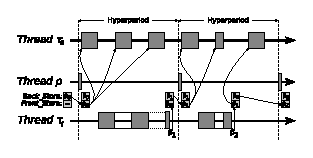
\includegraphics[scale=1.5]{figs/protocol2}
\caption{A suboptimal implementation. Left: Data flow from a fast
  thread to a slow thread. Right: Data flow from a slow thread to a
  fast thread}
\label{fig:protocol_thread}
\end{figure}

\subsection{Deterministic bridge exchangers}
\label{sec:DBX}
A more elegant and lightweight solution based on the connector
formalism is proposed. The central tenet of the connector approach is
that in a component based system, the communication constructs should
be separate from the computational components with interaction among
them taking place via well-defined APIs. From~\cite{mehta@icse00}:

\emph{Connectors mediate interactions among components: that is, they
  establish the rules that govern component interaction and specify
  any auxiliary mechanisms required.}

The code generation rules presented in the previous chapter are
specially well adapted to this notion, since the exchangers and
synchronizers that carry out communication and synchronization among
the various tasks are completely separate from the tasks
themselves. Furthermore, they can only be manipulated via the
precisely defined APIs that they expose. Thus, a modification of the
exchanger protected object is proposed as an efficient solution to the
problem of deterministic data flow in the context of AADL to Ada code
generation for a Ravenscar executive.

One of the main advantages of using a connector abstraction is the
clear separation between components and communication mechanisms,
which are generally two orthogonal concerns of a system. Data flow
presents an ideal case where the components are the participating
threads. By subsuming the functionality of the---above mentioned---
protocol into a connector any pollution of functional code with
communication logic is eliminated.

From the discussion on the protocol, it is apparent that two
distinctly different cases exist. One where a fast thread (or higher
frequency thread, or a thread with a smaller period) is the source of
the data flow towards a slow thread (or lower frequency thread, or a
thread with a smaller period). The other case is the opposite, i.e., a
slow thread is the source of a data flow towards a fast thread.

To implement each type of data flow, a separate type of connector is
needed. A connector that implements a data flow from a high-frequency
or faster thread to a low-frequency or slower thread is called a
\emph{stepper deterministic bridge exchanger}, or stepper DBX. The
converse connector, which implements a deterministic data flow from a
low-frequency or slower thread to a high-frequency or faster thread is
called a \emph{stagger deterministic bridge exchanger}, or stagger
DBX. Both types of connectors have an internal double buffer of the
same type as the data flow, called the \emph{back store} and
\emph{front store}. Both also provide a concurrency-safe API of
\texttt{Get\_Value} and \texttt{Set\_Value} procedures. Thus, both
types of DBX connectors are basically a specialized type of the
exchanger protected object as explained in Sec.~\ref{sec:dataports}.

An abstract overview of both types of connectors is given below. This
discussion is followed by details of how the modeling of these
deterministic data flows was added to the AADL, and how ARC supports
their automatic generation based on the model information available.

\subsubsection{Stepper Deterministic Bridge Exchanger}
This connector implements a deterministic data flow from a
high-frequency thread \ts to a low-frequency thread \tl. \ts computes
a new value and calls \texttt{Set\_Value} on the connector on each
job, which is read by \tl on each job via a call to the connector's
\texttt{Get\_Value} procedure. From the assumptions made on the system
it is known that in each mutual hyperperiod \plong, there will be
$r=P_{long}/P_{short}$ invocations of \texttt{Set\_Value} and one
invocation of \texttt{Get\_Value}, corresponding to the jobs of \ts
and \tl during said hyperperiod respectively. Also, at the start of
each \plong, it will be \texttt{Set\_Value} which will be invoked
first, as \ts has a higher priority. In order to implement the
deterministic data flow protocol, a stepper deterministic bridge
exchanger embeds buffer handling logic into \texttt{Set\_Value}, as
follows:

\begin{enumerate}
\item{On the first dispatch of \ts in every hyperperiod---i.e., on
  invocation number $i\in\mathbb{N}:i\times r+1$ of
  \texttt{Set\_Value}--- the procedure copies the \emph{back store}
  into the \emph{front store}, the data provided in the parameter of
  the \texttt{Set\_Value} procedure is discarded;}
\item{On the last dispatch of \ts in every hyperperiod---i.e., on
  invocation number $i\in\mathbb{N}:i\times r+r$ of
  \texttt{Set\_Value}---the procedure copies the data provided in the
  parameter of the \texttt{Set\_Value} procedure into the \emph{back
    store};}
\item{Every invocation of \texttt{Get\_Value} returns the \emph{front
    store} to the caller (the destination thread \tl)}
\end{enumerate}

The pseudocode for the \texttt{Set\_Value} procedure of a stepper DBX
is shown as Algorithm~\ref{algo:stepper_write}. It is called a
\emph{stepper} DBX because it \emph{steps over} a certain number of
inputs to the data flow, with only every $r^{th}$ data value copied
into the \emph{back store}.

\begin{algorithm}
\caption{\texttt{Set\_Value (\textbf{in} Data})}
\label{algo:stepper_write}
\SetKwInOut{D}{Data}
\SetKwInOut{r}{r}
\SetKwInOut{inv}{Invocation}
\inv{static integer initialized to 0}
\D{input for dataflow, provided by source thread}
\r{integer corresponding to $P_{long}/P_{short}$}
\SetLine
\Begin{
    \SetNoline
    Invocation $\leftarrow$ Invocation + 1\\
    \If{Invocation = 1}{
      Front\_Store $\leftarrow$ Back\_Store\\
    }
    \If{Invocation = r}{
      Back\_Store $\leftarrow$ Data\\
      Invocation $\leftarrow$ 0\\
    }
    \Return\\
}
\end{algorithm}

\subsubsection{Stagger Deterministic Bridge Exchanger}
This connector implements a deterministic data flow from a
low-frequency thread \tl to a high-frequency thread \ts. \tl computes
a new value and calls \texttt{Set\_Value} on the connector on each
job, which is read by \ts on each job via a call to the connector's
\texttt{Get\_Value} procedure. From the assumptions made on the
system, it is known that in each mutual hyperperiod \plong, there will
be $r=P_{long}/P_{short}$ invocations of \texttt{Get\_Value} and one
invocation of \texttt{Set\_Value}, corresponding to the jobs of \tl
and \ts during said hyperperiod respectively. Also, at the start of
each \plong, it will be \texttt{Get\_Value} which will be invoked
first, as \ts has a higher priority. Thus, a stagger deterministic
bridge exchanger embeds buffer handling logic into
\texttt{Get\_Value}, as follows:

\begin{enumerate}
\item{On the first dispatch of \ts in every hyperperiod---i.e., on
  invocation number $\forall i\in\mathbb{N}:i\times r+1$ of
  \texttt{Get\_Value}---the procedure copies the \emph{back store} into the
  \emph{front store};}
\item{Every invocation of \texttt{Get\_Value} returns the data in the
  \emph{front store};}
\item{Every invocation of \texttt{Set\_Value} copies the data provided
  by the source thread as the parameter of the procedure into the
  \emph{back store}.}
\end{enumerate}

The pseudocode for the \texttt{Set\_Value} procedure of a stagger DBX
is shown as Algorithm~\ref{algo:stagger_read}. It is called a
\emph{stagger} DBX because it \emph{staggers} on a data flow value a
certain number of times before getting a new one.

\begin{algorithm}
\caption{\texttt{Get\_Value (\textbf{out} Data})}
\label{algo:stagger_read}
\SetKwInOut{D}{Data}
\SetKwInOut{r}{r}
\SetKwInOut{inv}{Invocation}
\inv{static integer initialized to 0}
\D{output for dataflow, sent to destination thread}
\r{integer corresponding to $P_{long}/P_{short}$}
\SetLine
\Begin{
    \SetNoline
    Invocation $\leftarrow$ Invocation + 1\\
    \If{Invocation = 1}{
      Front\_Store $\leftarrow$ Back\_Store\\
    }
    \If{Invocation = r}{
      Invocation $\leftarrow$ 0\\
    }
    Data $\leftarrow$ Front\_Store\\
    \Return\\
}
\end{algorithm}

\subsubsection{Advantages of the approach}
There are numerous advantages of this approach. It allows a clean
decoupling of the functional and non-functional code in the system;
with the functional code being that which is implemented in the
callbacks of the threads and the non-functional being their temporal
characteristics as well as the communication infrastructure. It also
reduces the number of threads in the system as there is no need for
extra threads to handle the protocol logic, it is done within the
communication construct itself (the exchanger protected
object). Furthermore, with the automatic generation of these
connectors, as is explained in the following section, it allows the
reuse of the threads' functional code, and easier redimensioning in
case of a redesign.

\subsection{Integration into tooling}
\label{sec:implem}
The two types of DBX connectors have been integrated into the ARC code
generator, and is represented in the AADL via connections between data
ports. Towards this end, there needs to be a very minor modification
to the AADL in the form of an additional property, which specifies
that a connection between two data ports is a deterministic one. The
other part is the actual generation of Ada code for the special
protected object.

In the original mapping, AADL threads are transformed to Ada tasks,
and each \texttt{in data port} and \texttt{in out data port} in the
features section of the thread is transformed to an \emph{exchanger}
protected object. As stated, an exchanger is an Ada protected object
with an internal private data area, and two concurrency-safe access
procedures to get and set the internal data. The basic exchanger
immediately copies the data provided as the \texttt{Set\_Value}
procedure's parameter to the internal data, this is the data value
that is returned upon the next invocation of the \texttt{Get\_Value}
procedure. This implementation is perfectly valid for applications
where deterministic communication is not a requirement, e.g., a moving
map display where the display thread has a period of 500 ms and the
data from the GPS is refreshed every 100 ms. A slight amount of
non-determinism in this application would be neither noticeable nor
critical.

Both types of deterministic bridge exchangers have been implemented as
generic Ada packages within the library \texttt{ravenscar\_lib}. The
only element within these packages is a protected object instance that
implements the protocol according to
Algorithms~\ref{algo:stepper_write} and~\ref{algo:stagger_read}. Both
generic packages---which are named \texttt{Stepper\_DBX} and
\texttt{Stagger\_DBX}---have a number of instantiation parameters
which configure the exchanger, these parameters are:

\begin{description}
\item[Priority\_P:]{The ceiling priority for its protected object;}
\item[Factor\_P:]{The \emph{stepper factor} or \emph{stagger factor},
  $r=T_{long}/T_{short}$;}
\item[Data\_Type\_P:]{The data classifier (type) of the data ports
  involved.} 
\end{description}

The specification of the generic package that implements a stepper DBX
connector is given in Listing~\ref{lst:DBX_spec}. The generic package
only has a protected object instance that serves as the exchanger. The
specification for a stagger DBX connector is similar.

\begin{minipage}{0.45\linewidth}
\lstset{language=ada}
\begin{lstlisting}[label=lst:DBX_spec, caption=Specification of the Stepper DBX connector]
generic
  Priority_P : System.Any_Priority;
  Factor_P : Integer;
  type Data_Type_P is private;
package Stepper_DBX is
  protected Stepper_DBX_Instance is
    
    procedure Set_Value (
      D : in Data_Type_P
    );
    
    procedure Get_Value (
      D : out Data_Type_P;
      F : out Boolean
    );

  private
    pragma Priority (Priority_P);
    Back_Store : Data_Type_P;
    Front_Store : Data_Type_P;
    Invocation : Integer := 0;
    Fresh : Boolean := False;
  end Stepper_DBX_Instance;
end Stepper_DBX;
\end{lstlisting}
\end{minipage}
\hspace{5mm}
\begin{minipage}{0.45\linewidth}
\lstset{language=ada}
\begin{lstlisting}[label=lst:DBX_body, caption=Stepper DBX connector
    \texttt{Set\_Value} procedure]




procedure Set_Value (
  D : in Data_Type_P
) is
begin
  Invocation := Invocation + 1;
  if Invocation = 1 then
    Front_Store := Back_Store;
    Fresh := True;
  end if;
  if Invocation = Factor then
    Back_Store := D;
    Invocation := 0;
  end if;
  return;
end Set_Value;




--
\end{lstlisting}
\end{minipage}

The \texttt{Front\_Store} and \texttt{Back\_Store} private variables
serve as the internal buffers for the data. As is apparent from
Listing~\ref{lst:DBX_body}, the code of the \texttt{Set\_Value}
procedure follows the algorithm as described for the adherence to the
data flow protocol. The instantiation parameter \texttt{Factor\_P}
determines the ratio between the job frequency of both tasks and can
be used to determine the beginning of a new mutual hyperperiod. The
code for the stagger DBX is similar, and for reference its
specification is shown in Listings~\ref{lst:stagger_spec} and the
implementation of its \texttt{Get\_Value} procedure in
Listing~\ref{lst:stagger_get}. For every deterministic communication
connection in the AADL model, an appropriately named and parametrized
stepper or stagger exchanger package is instantiated in the
\texttt{Local\_Comm} package, with the appropriate API generated in
the two participating threads' functional unit packages.

\begin{minipage}{0.45\linewidth}
\lstset{language=ada}
\begin{lstlisting}[label=lst:stagger_spec, caption=Specification of the Stagger DBX connector]
generic
  Priority_P : System.Any_Priority;
  Factor_P : Integer;
  type Data_Type_P is private;

package Stagger_DBX is

  protected DBX_Instance is
      
    procedure Set_Value (
      D : in Data_Type_P
    );

    procedure Get_Value (
      D : out Data_Type_P; 
      F : out Boolean
    );
    
    procedure Initialize (
      D : in Data_Type_P
    );
  
  private
    pragma Priority (Priority_P);
    Fresh       : Boolean := False;
    Factor      : Integer := Factor_P;
    Invocation  : Integer := 0;
    Back_Store  : Data_Type_P;
    Front_Store : Data_Type_P;
  end DBX_Instance;

end Stagger_DBX;
\end{lstlisting}
\end{minipage}
\hspace{5mm}
\begin{minipage}{0.45\linewidth}
\lstset{language=ada}
\begin{lstlisting}[label=lst:stagger_get, caption=Stagger DBX connector
    \texttt{Get\_Value} procedure]







procedure Get_Value (
  D : out Data_Type_P; 
  F : out boolean
) is
begin
  Invocation := Invocation + 1;
  if Invocation = 1 then
    Front_Store := Back_Store;
    Fresh := True;
  end if;
  if Invocation = Factor then
    Invocation := 0;
    Fresh := False;
  end if;
  D := Front_Store;
  F := Fresh;
  return;
end Get_Value;






--
\end{lstlisting}
\end{minipage}

In order to declare a connection between two data ports to be
deterministic, a new AADL property is introduced to the Ravenscar
property set. The property \texttt{Is\_DBX} is of type boolean and
applies to data connections, i.e., connections between two data
ports. If this property is set to \texttt{True}, it stipulates that
the data transfer is to be deterministic over this connection. ARC
verifies that for every DBX connection the following conditions hold:

\begin{enumerate}
\item{The connection must be between data ports;}
\item{Both threads must be periodic;}
\item{The period of one thread must be an integral multiple of the
  period of the other.}
\end{enumerate}

Whether a stepper or a stagger DBX is instantiated depends on whether
the source thread has the shorter period or not. In addition to the
instantiation of the DBX connector, stub procedures are generated in
the functional unit packages of both threads which allow easy access
to the DBX. On the side of the source thread a stub procedure named
\texttt{Set\_<Port\_Name>} is generated. On the side of the
destination thread a stub named \texttt{Get\_<Port\_Name>} is
generated, the same as for normal data port connections. These
procedures simply call the \texttt{Set\_Value} and \texttt{Get\_Value}
procedures of the actual exchanger. One such transformation is shown
in Fig.~\ref{fig:transformation}. This creates a complete
deterministic communication framework and also generates an API to
access it. This aids the designer since he now has to focus on only
the functional part. Among the advantages of this approach are:

\begin{itemize}
\item{Eliminates impact from system architecture to functional
  code. All protocol information is embedded in the connector. The
  functional part need only interact with the generated API;}
\item{Reduces programmer effort and errors through the use of
  automatic code generation;}
\item{Aids in the certification process for onboard software. This
  point will be explained in the next section.}
\end{itemize}

\begin{figure}
\centering
\includegraphics[scale=1.8]{figs/transform}
\caption{Code generation from AADL with a stepper DBX between two
  tasks}
\label{fig:transformation}
\end{figure}

\subsection{Example of utilization}
To illustrate the use of the DBX connectors, consider the example of a
simple control system that contains one periodic thread to read the
value of a sensor, one periodic thread that performs some kind of
computation or data fusion on the value read, and one sporadic thread
that is an alarm for non-nominal occurrences within the
system. Imagine also that the sensor thread is the highest priority
thread, the alarm thread is at an intermediate priority and the data
fusion thread is the lowest priority thread. The system is shown in
Fig.~\ref{fig:control_simple}. The \texttt{Sensor\_A} thread has a
period of 20 ms and is at the highest priority, the sporadic thread
\texttt{Alrm\_1} has an inter-arrival time of 30 ms and so is at an
intermediate priority, finally, thread \texttt{Data\_Fusion} is
periodic with a period of 40 ms, and so is the lowest priority thread.

\begin{figure}
\centering
\includegraphics[scale=0.6]{figs/control}
\caption{The example system with two periodic and one sporadic thread}
\label{fig:control_simple}
\end{figure}

Thus, during every mutual hyperperiod of \texttt{Sensor\_A} and
\texttt{Data\_Fusion}, the former is dispatched twice whereas the
latter is dispatched once, \texttt{Alrm\_1} may be dispatched at any
point in time. In order to simulate a situation where
non-deterministic communication would be harmful, consider that the
threads perform the following computations:

\begin{description}
\item[Sensor\_A:]{Increments and sends an integer over the port
  \texttt{outp} at every dispatch. At every $8^{th}$ dispatch it sends
  an event over event port \texttt{launch\_alrm\_1}, which launches
  the thread \texttt{Alrm\_1}, this is to simulate environmental
  stimuli;}
\item[Data\_Fusion:]{Receives an integer over the port \texttt{inpA}
  at every dipatch. If the integer received is not one more than the
  last one received then prints an error statement, otherwise it does
  nothing;}
\item[Alarm\_1:]{Goes into a busy loop for 22 ms every time it is
  dispatched over \texttt{event port launch\_A}.}
\end{description}

Given these functional specifications for the various threads, it is
easy to see that once every $8^{th}$ dispatch of the thread
\texttt{Sensor\_A}, the data flow between it and
\texttt{Sensor\_Fusion} will be disturbed due to the job of the alarm
thread. Graphically, this can be approximated as shown in
Fig.~\ref{fig:det_breach_simple}. It is apparent that in the
\emph{first} hyperperiod, it is the first job of \texttt{Sensor\_A}
that writes to \texttt{Data\_Fusion}, whereas in the second
hyperperiod, it is the \emph{second} job of \texttt{Sensor\_A} that
writes, because the thread \texttt{Alrm\_1} has run for a sufficient
amount of time that the periodic dispatch of \texttt{Sensor\_A} is now
possible, thus letting it run before the job of
\texttt{Data\_Fusion}. This problem can be simply fixed by setting the
\texttt{Is\_DBX} property to \texttt{True} for the data connection
between the ports \texttt{outp} and \texttt{inpA}. This will result in
the data flow as shown in Fig.~\ref{fig:det_no_breach}. This is
possible because now a stepper DBX has been instantiated in the
\texttt{Local\_Comm} package to handle the data flow between these two
threads. The \emph{factor} for this stepper DBX is computed to be 2
(40/20), and it is given the appropriate ceiling priority to ensure
deadlock-free execution.

\begin{figure}
\centering 
\includegraphics[scale=0.75]{figs/control_simple_breach}
\caption{Data flow determinism breached}
\label{fig:det_breach_simple}
\vspace{5mm}
\includegraphics[scale=0.75]{figs/control_simple_nobreach}
\caption{Data flow determinism with deterministic exchanger}
\label{fig:det_no_breach}
\end{figure}

\subsection{Verification}
\label{sec:verif}
Safety-critical software such as fly-by-wire, computer controlled
braking of cars and railway signaling systems have a number of very
restrictive certification constraints. For software systems deployed
aboard aircraft, the DO-178B standard is the currently accepted
one. Although the current version of the standard includes only tests
as a means to obtaining certification, it does not rule out the use of
either formal verification or proofs as means of certification of
certain aspects of the system. In addition, the new version of the
standard, DO-178C, includes an annex that specifically addresses the
need for a methodology of using verification or proofs in lieu of
exhaustive tests as certification artifacts.

It is within this context that the current section provides a
verification methodology for the DBX connectors, specifically, the
claim that they \emph{always} provide the envisaged deterministic
communication (given that the system hypotheses hold). The
verification is carried out with the LOTOS (Language of Temporal
Order Specification) language~\cite{bolognesi@cnis87} using the CADP
toolbox from INRIA Rh\^one-Alpes~\cite{garavel@cav07}. Even though the
following paragraphs do provide a short overview of LOTOS, the
interested reader is referred to one of a number of
tutorials~\cite{bolognesi@cnis87, logrippo@cnis92} for a deeper
understanding of the language.

\subsubsection{Overview of LOTOS}
LOTOS (Language of Temporal Order Specifications) is a process
algebraic formal description technique inspired by
CCS~\cite{milner-cc} and CSP~\cite{hoare@cacm78}. It uses the concept
of observable actions carried out by independent processes. Processes
synchronize upon actions; these actions are taken over \emph{gates}
and may potentially involve an exchange of data between the gates of
the synchronized processes.

The actions a LOTOS process can undertake are written in the form
\texttt{a; b; c} which means the process engages in \texttt{a},
followed by \texttt{b}, and finally \texttt{c}. Actions of the sort
\texttt{g!x} signify that an action is taken on \emph{gate} \texttt{g}
and offers \texttt{x} as the associated data. This action would need
to be \emph{synchronized} with a corresponding action of the sort
\texttt{h?x} which signifies an action on gate \texttt{h} receiving
data \texttt{x}, this is akin to a rendezvous. Any number of LOTOS
processes can be put in parallel using a number of different
operators; the \texttt{[]} operator, signifying an exclusive or choice
of action between the two processes; the \texttt{|[gate\_list]|}
operator, signifying synchronization on the gates given in the list;
the \texttt{||} operator, signifying a synchronization on \emph{all}
gates; or the \texttt{|||} operator, signifying an independent
interleaving of the actions of the two participating processes.

LOTOS allows for verification by carrying out an exhaustive state
space exploration of the provided specification, this gives \emph{all}
possible outcomes and sequences of events that the system may engage
in. If, in this state space exploration, no state is found that
violates a given condition---the one being tested for---then the
system can be considered to be sound. An example of a simple LOTOS
specification of two processes communicating over a channel is given
in Listing~\ref{lst:lotos_ex}, the resulting labelled transition
system (LTS) which is constructed via the state space exploration is
shown in Fig.~\ref{fig:lotos_ex}. The specification puts the three
processes---\texttt{Producer}, \texttt{Consumer} and
\texttt{Channel}--- in parallel using the selected composition
operator \texttt{|[gate\_list]|}. The definitions of the behavior of
each process is given in the \kw{where} section.

\begin{minipage}{\listingwidth}
\lstset{language=lotos}
\begin{lstlisting}[label=lst:lotos_ex, caption=An example of a LOTOS
    specification]
specification IO_System [pc1, pc2, cc1, cc2] : exit behavior
  Producer [pc1, pc2]
    |[pc1, pc2]|
  Channel [pc1, pc2, cc1, cc2]
    |[cc1, cc2]|
  Consumer [cc1, cc2]

where

  process Producer [pc1, pc2] : exit :=
    pc1; pc2; exit
  endproc

  process Consumer [cc1, cc2] : exit :=
    cc1; cc2; exit
  endproc

  process Channel [pc1, pc2, cc1, cc2] : exit :=
    pc1; pc2; cc1; cc2; exit
  endproc
endspec
\end{lstlisting}
\end{minipage}

\begin{figure}
\centering
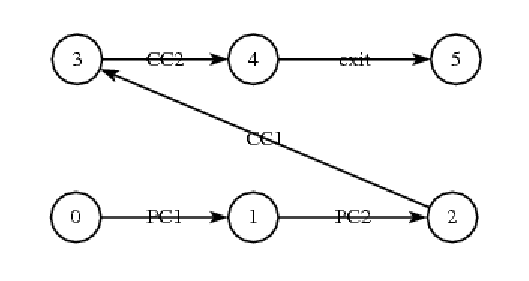
\includegraphics[scale=1]{figs/ex1}
\caption{The resulting labelled transition system}
\label{fig:lotos_ex}
\end{figure}

\subsection{Connector and thread specifications in LOTOS}
In order to verify the correct behavior of the connectors, the
exchanger as well as the two participating threads need to be
converted to LOTOS processes, putting them in parallel with the
appropriate composition operators then gives the resulting labelled
transition system. The source and destination threads' LOTOS processes
engage in actions named \texttt{WRITE\_<Port\_Name>} and
\texttt{READ\_<Port\_Name>} respectively, from now on abbreviated to
\texttt{READ} and \texttt{WRITE}. The source thread offers a natural
number as the data type with each \texttt{WRITE} action, and the
destination thread accepts it. This natural number is the
\emph{instance} of data flow being sent; the first job will offer $1$,
the second job $2$, and so on. These two actions are synchronized with
by exchanger's process, which models the data flow protocol, and acts
as a channel between the two threads.

The specification is built in such a way that in case of a reception
of an unexpected data flow value at the destination thread, an error
action is generated. Thus, inspection of the list of actions resulting
from the LTS generation can determine whether the determinism of data
flow has been preserved. ARC contains an auxiliary code generator for
LOTOS as well. This auxiliary code generator traverses the RMM model
and generates a LOTOS specification corresponding to the system.

The generated LOTOS process specification of a DBX connector can
engage in actions \texttt{READ} or \texttt{WRITE}, which correspond to
the \texttt{Get\_Value} and \texttt{Set\_Value} procedures exposed by
the Ada Ravenscar implementation. Both of these actions are composed
together with the \texttt{[]} choice operator, meaning that an
``idle'' exchanger may engage in one or the other action. The
\texttt{WRITE} action accepts a data offer, which represents the
instance of the data flow. Similarly, the \texttt{READ} action offers
data, which is concordant with the output parameter of the procedure
in the Ada exchanger. The process specification has two variables
\texttt{Store\_0} and \texttt{Store\_1} which stand for the back store
and front store respectively. These two variables are manipulated
according to the algorithms given and represent the internal buffers
of the exchanger. Finally, the exchanger has two variables named
\texttt{Inv} and \texttt{Factor} which keep track of the invocation
count and the ratio between the periods of the two participated
threads. The stepper exchanger generated automatically for the example
given in the previous section is shown in
Fig.~\ref{fig:lotos_stepper}. Preemption of a thread \emph{inside} an
exchanger is not modeled---the \texttt{READ} and \texttt{WRITE}
actions are unique---because the purpose is the verification of the
data flow. Even though during the actual system's execution, a task
\emph{may} be preempted while it is inside an exchanger's procedure,
thanks to the priority ceiling protocol, it will never be preempted by
another task that may access the same exchanger (because the ceiling
priority of the exchanger, and consequently the task inside it, would
be at least equal to that of the other task). Thus, the procedures of
the exchanger can be considered atomic \emph{with respect to the other
  procedures and entries of the same exchanger}. In this context, the
actions \texttt{READ} and \texttt{WRITE} can be considered an accurate
approximation of the behavior of the system, and both of these actions
can be thought of as occurring at the moment the task \emph{returns}
from the exchanger procedure, and has had the desired effect.

\begin{figure}
\centering
\includegraphics[angle=90, scale=0.70]{figs/stepper_code}
\caption{LOTOS specification for a process modeling a stepper
  exchanger}
\label{fig:lotos_stepper}
\end{figure}

The specification of the stepper exchanger states that on the
\emph{first} invocation of the \texttt{WRITE} action,
\texttt{Store\_0} is promoted to \texttt{Store\_1} and it is given a
non-valid value (100 in this case). On the \emph{last} invocation of
the \texttt{WRITE} action, the provided value is written to
\texttt{Store\_0}. For all other invocations, the provided value is
discarded and both stores keep their existing values. At each
invocation of the \texttt{READ} action, the value of \texttt{Store\_1}
is returned and it is set to an invalid value (100 in this case).

The LOTOS specifications for the two threads of the example are given
in Fig.~\ref{fig:lotos_proc_code}. The LOTOS process
\texttt{Sensor\_A} models the source thread, and takes actions to
write to the gate \texttt{WRITE\_Data\_Fusion\_inpA} at the start of
every mutual hyperperiod, which is represented by the action on gate
\texttt{FRAME\_START}. Three hyperperiods are modeled, at the start of
each of which it is \texttt{Sensor\_A} which takes the write action,
followed by an \emph{interface action} which enables the potential
execution of the \texttt{Data\_Fusion} thread. Finally,
\texttt{Sensor\_A} writes again to the exchanger and signals its end
of activity for the hyperperiod by engaging in
\texttt{FRAME\_END}. The LOTOS process \texttt{Data\_Fusion} models
the behavior of the destination thread. It is at a lower priority so
at every single hyperperiod start---action \texttt{FRAME\_START}---it
waits for the interface action from the \texttt{Sensor\_A} thread,
following which it engages in its \texttt{READ} action. This
particular example runs for three hyperperiods, at each of which
\texttt{Data\_Fusion} tests the value of the received data with the
read action. If the data conforms to the value expected, it moves on,
otherwise it engages in the \texttt{ERR} action followed by the
special LOTOS action \texttt{stop}, which halts the system. Thus the
presence of the \texttt{ERR} action points to an error in the data
flow of the system. Similar to the model for exchangers, preemption of
threads is not modeled because the aspect of interest in this
verification exercise is the data flow. The actions taken by the
thread specifications are those that represent reading data from an
exchanger, writing data to one, the starts and ends of mutual
hyperperiods and the ``interface'' actions which enable a
lower-priority thread by signaling that the synchronously-released
higher-priority thread has finished execution. The object of interest
is simply the \emph{order} in which the events that these actions
represent take place.

\begin{figure}
\centering
\includegraphics[scale=0.7, angle=90]{figs/lotos_proc_code}
\caption{LOTOS specification for the two threads}
\label{fig:lotos_proc_code}
\end{figure}

The system---the LOTOS processes representing the two threads
\emph{and} the DBX exchanger---is composed together using the
appropriate parallel composition operators. The CADP toolbox is then
used to generate the labelled transition system corresponding to
it. The LTS generated---and reduced with branching equivalence---from
the example being followed till now is shown in
Fig.~\ref{fig:lts_ex1}. The total number of states explored in this
example is 39, and the total number of transitions is 43, the
transitions include:

\begin{verbatim}
FRAME_START 
WRITE_DATA_FUSION_INPA !1 
WRITE_DATA_FUSION_INPA !2 
READ_DATA_FUSION_INPA !0 
FRAME_END 
WRITE_DATA_FUSION_INPA !3 
WRITE_DATA_FUSION_INPA !4 
READ_DATA_FUSION_INPA !2 
WRITE_DATA_FUSION_INPA !5 
WRITE_DATA_FUSION_INPA !6 
READ_DATA_FUSION_INPA !4 
\end{verbatim}

There are a large number of ``hidden'' transitions that are not given
in the above list, they have been optimized out by the CADP model
checker. It is obvious that no \texttt{ERR} action has occurred and
the system has performed correctly for all three hyperperiods, with
all possible permutations of the legal scheduling of the two
threads. From Fig.~\ref{fig:lts_ex1}, a few characteristics of the
system can be deduced. The three diamond shaped configurations are the
three hyperperiods of the two participating threads. At the start of
\emph{every} hyperperiod, marked by the \texttt{FRAME\_START} action,
the thread \texttt{Sensor\_A} carries out the write action first. This
may be followed by either the second write action of the
\texttt{Sensor\_A} thread \emph{or} the read action of the
\texttt{Data\_Fusion} thread. This corresponds to the situations where
a sporadic thread may or may not interrupt the dispatch of
\texttt{Data\_Fusion} until the next dispatch of \texttt{Sensor\_A}.

To enable the automatic generation of LOTOS verification code for an
AADL model, the property \texttt{Frames\_To\_Verify} must be set to a
non-zero value on the process component that contains the threads and
connections which are to be modeled. The default value of this
property is 0, which signifies that verification code generation is
not requested. The example presented previously had LOTOS code
generated for three hyperperiods, thus the process that contained the
threads \texttt{Sensor\_A} and \texttt{Data\_Fusion} had the property
association \texttt{Frames\_To\_Verify => 3}.

\begin{figure}
\centering
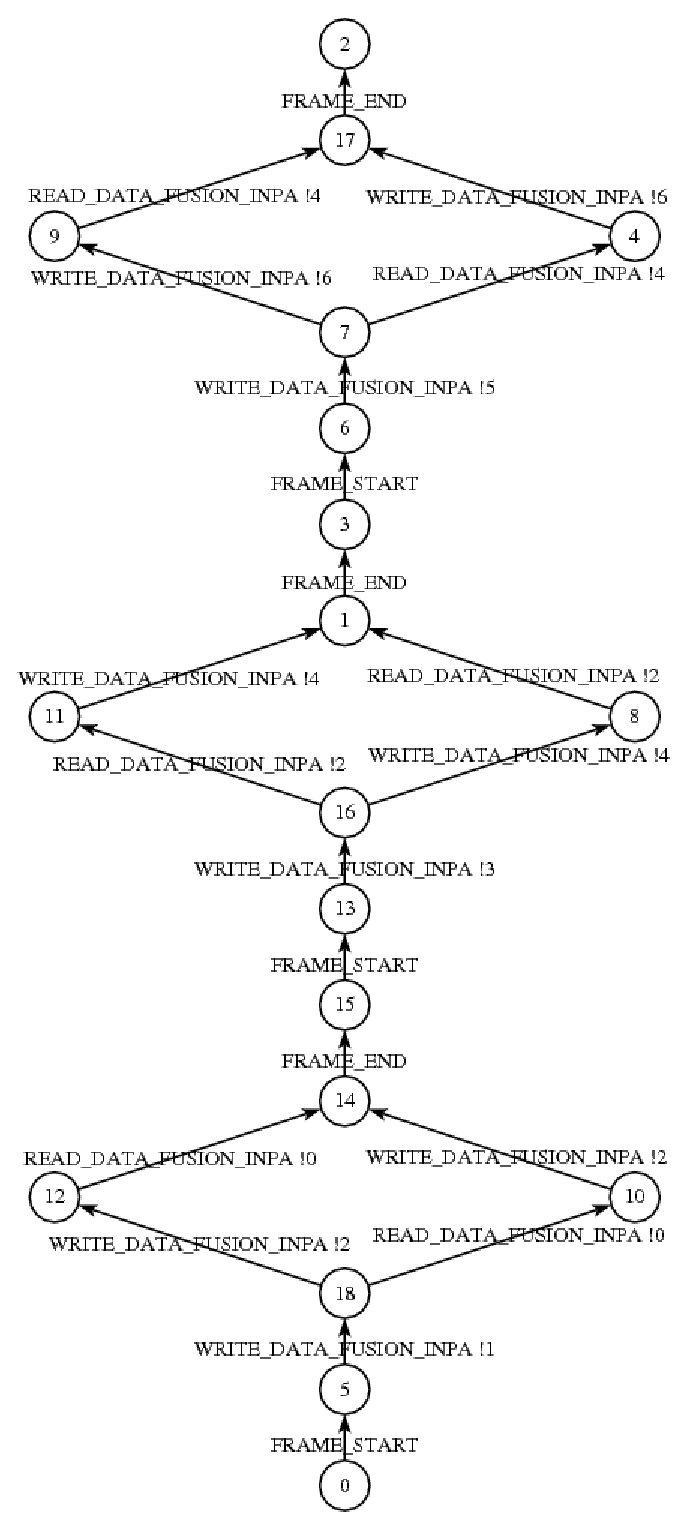
\includegraphics[scale=0.8]{figs/lotos_lts_ex1}
\caption{The labelled transition system generated by CADP from the example}
\label{fig:lts_ex1}
\end{figure}

\newpage
\begin{comment}
\begin{sideways}
\lstset{language=lotos, frame=none}
\begin{lstlisting}[label=lst:lotos_stepper, caption=LOTOS
    specification for a process modeling a stepper exchanger]
process STEPPER_Data_Fusion_inpA[READ_Data_Fusion_inpA, WRITE_Data_Fusion_inpA] (Inv, Factor, Store_0, Store_1 : NAT) : noexit :=
  WRITE_Data_Fusion_inpA?x:NAT;
  (
    [Inv eq 1] -> STEPPER_Data_Fusion_inpA[READ_Data_Fusion_inpA, WRITE_Data_Fusion_inpA] (Inv+1, Factor, 100, Store_0)
      []
    [Inv eq Factor] -> STEPPER_Data_Fusion_inpA[READ_Data_Fusion_inpA, WRITE_Data_Fusion_inpA] (1, Factor, x, Store_1)
      []
    [(Inv ne 1) and (Inv ne Factor)] -> STEPPER_Data_Fusion_inpA[READ_Data_Fusion_inpA, WRITE_Data_Fusion_inpA] (Inv+1, Factor, Store_0, Store_1)
  )
    []
  (
    READ_Data_Fusion_inpA!Store_1; STEPPER_Data_Fusion_inpA[READ_Data_Fusion_inpA, WRITE_Data_Fusion_inpA] (Inv, Factor, Store_0, 100)
  )
endproc
\end{lstlisting}
\end{sideways}

\newpage
\begin{sideways}\centering
\lstset{frame=none, language=lotos}
\begin{lstlisting}[label=lst:lotos_thread_procs, caption=LOTOS
    specifications for the two threads]
process Sensor_A [FRAME_START, FRAME_END, ERR, WRITE_Data_Fusion_inpA, Interface_Sensor_A_Data_Fusion] : noexit :=
  FRAME_START; WRITE_Data_Fusion_inpA!(1); Interface_Sensor_A_Data_Fusion; WRITE_Data_Fusion_inpA!(2); FRAME_END; 
  FRAME_START; WRITE_Data_Fusion_inpA!(3); Interface_Sensor_A_Data_Fusion; WRITE_Data_Fusion_inpA!(4); FRAME_END; 
  FRAME_START; WRITE_Data_Fusion_inpA!(5); Interface_Sensor_A_Data_Fusion; WRITE_Data_Fusion_inpA!(6); FRAME_END; 
  stop
endproc

process Data_Fusion [FRAME_START, FRAME_END, ERR, READ_Data_Fusion_inpA, Interface_Sensor_A_Data_Fusion] : noexit :=
  FRAME_START; Interface_Sensor_A_Data_Fusion; READ_Data_Fusion_inpA?Data_Fusion_inpA_V:NAT; 
  (
    [not (Data_Fusion_inpA_V eq 0)] -> ERR; stop
      []
    [Data_Fusion_inpA_V eq 0]-> exit
  )
  >>
  FRAME_END; 
  FRAME_START; Interface_Sensor_A_Data_Fusion; READ_Data_Fusion_inpA?Data_Fusion_inpA_V:NAT; 
  (
    [not (Data_Fusion_inpA_V eq 2)] -> ERR; stop
      []
    [Data_Fusion_inpA_V eq 2]-> exit
  )
  >>
  FRAME_END; 
  FRAME_START; Interface_Sensor_A_Data_Fusion; READ_Data_Fusion_inpA?Data_Fusion_inpA_V:NAT; 
  (
    [not (Data_Fusion_inpA_V eq 4)] -> ERR; stop
      []
    [Data_Fusion_inpA_V eq 4]-> exit
  )
  >>
  FRAME_END; 
  stop
endproc
\end{lstlisting}
\end{sideways}
\newpage
\end{comment}

\subsection{Application to Certification}
DO-178B~\cite{do178b} is a widely accepted and applied standard for
avionics software. It divides onboard software into one of five
categories according to its safety requirements. These levels are
given in Table~\ref{table:do178b_cats}. Level A software is of highest
criticality, and it is at this level that all control software must be
certified. The standard stipulates that Level A certified software
undergo Modified Condition/Decision Coverage (MCDC) testing. This code
coverage method requires a test case to verify each condition that can
affect the outcome of a decision. A compound condition such as
\texttt{if(a>0 \&\& b<5)} would result in four MCDC test cases
with $a\le 0$, $a>0$, $b<5$ and $b\ge 5$. Also, it is not patently
clear how test cases such as these could even be used to completely
test application software that has sporadic threads and environmental
stimuli. Due to the temporally unpredictable nature of the system, no
amount of testing could provide complete coverage from the
point-of-view of arbitrarily dispatched sporadic threads and the
consequences of their load on the system.

Also, generating such test cases by hand is not feasible. Level A
certification thus requires instrumented compilers to identify and
generate test cases. However, for complex software the number of test
cases generated may be very large and thus testing becomes
expensive. Verified exchangers for deterministic communication can
reduce this cost by providing verification artifacts in support of
certification. This can potentially allow the certification authority
to forego MCDC coverage of the exchangers as their behaviour has been
formally verified and all conditions/decisions examined thanks to the
exhaustive state-space search. In fact, the UK defence software
standard Def Stan 00-55~\cite{uk-def-stan} promotes proof of
correctness in the design rather than debugging. Research has shown
that there is a correlation between both
approaches~\cite{gasperoni@ae02}.

The automatic generation of the LOTOS specifications for exchangers as
well as all threads in the system that participate in deterministic
communication greatly aids in obtaining these ``certification
artifacts'' and eases a lot of load that would otherwise be leveraged
upon the development process, with its attendant increases in cost,
time-to-market and complexity. Translations of AADL to process
algebraic specifications have also been used to determine
schedulability of the system~\cite{sokolsky@ipdps06}.

\begin{table}
\centering
{\footnotesize
\begin{tabular}{|l|l|l|}
\hline
\textbf{Software level}&\textbf{Failure condition}&\textbf{Outcome}\\
\hline
Level A & Catastrophic & Death or injury\\
Level B & Hazardous/Severe-major & Injury\\
Level C & Major & Unsafe workload\\
Level D & Minor & Increased workload\\
Level E & No effect & None\\
\hline
\end{tabular}
}
\caption{DO-178B Safety Criticality Levels~\cite{gasperoni@ae02}}
\label{table:do178b_cats}
\end{table}

\section{Higher-order deterministic connectors}
This section presents an extension of the DBX connectors for
higher-order buffering. The basic DBX connectors presented in the
previous section provide only the values sampled from the last job of
the \emph{previous} hyperperiod. Consider, on the other hand, a
$2^{nd}$ order filter of the following form
(from~\cite{halbwachs@ieee91}:

\begin{displaymath}
H(z) = \frac{az^2 + bz + c}{z^2 + dz + e}
\end{displaymath}

The output of this filter, in the form $H(z)x$ can be written as:

\begin{displaymath}
y = ax + (bx-dy)z^{-1} + (cx-ey)z^{-2}
\end{displaymath}

Since the system is expressed in z-transform equations, it signifies
that values of $x$ that are multiplied by $z^{-1}$ is the last
deterministically sampled value of $x$. Similarly, values of $x$
multiplied by $z^{-2}$ is taken as the second-to-last
deterministically sampled value of $x$, and so on. These types of
systems can be implemented in an exceedingly simple manner using
synchronous and cyclic techniques:

\begin{description}
\item[Lustre/SCADE Suite:]{$z^{-1}$ when multiplied by $x$ would be
  equal to a \kw{pre}\texttt{(x)} and those with $z^{-2}$ would be
  equal to a \kw{pre}\texttt{(}\kw{pre}\texttt{(x))};}
\item[Simulink:]{It provides a standardized block called a
  ``zero-order hold'', cascading more than one in series would achieve
  the same effect, i.e., staggering the output value a certain number
  of times compared to the input value.}
\end{description}

Implementing these types of higher-order systems in the context of a
process-based executive with preemption and sporadic threads, however,
is not so simple. Fortunately, the approach described in the previous
section can be intuitively extended to provide the ideal constructs
for implementing such data flow. If the source of the data flow---$x$
in this case---is one periodic thread, and the destination is another,
then there can be two cases:

\begin{description}
\item[Both have same periods:]{This eliminates the problem, since it
  will be known \emph{\`a priori} which thread has the higher
  priority, and thus it will be known which one will execute first
  when both are released. The data flow becomes automatically
  determnistic;}
\item[Both threads have different periods:]{In this case, one thread's
  period should be an integral multiple of the other's, and a similar
  problem arises as described in the previous section.}
\end{description}

In order to describe such a data flow in AADL, a new property---named
\texttt{Hyperperiod\_Age} of type integer---has been defined which is
applied to AADL connections. For a connection that has the
\texttt{Is\_DBX} property set to true, this property gives the
\emph{age} of the hyperperiod from which to sample the data. Its
default value is 1, in which case the behavior becomes that of a
simple DBX connector. A value of 2 for the \texttt{Hyperperiod\_Age}
property would provide data from the last job of the second-to-last
hyperperiod of the source thread (in effect giving the value of
$z^{-2}$).

The implementation of higher-order DBX connectors in Ada is
conceptually similar to that of simple or first-order DBX, with the
following modifications:

\begin{itemize}
\item{Instead of a generic package, their protected object types are
  generated in the \texttt{Task\_Features}, this is due to the
  differences in behavior;}
\item{Instead of a back and front store implemented as separate
  variables, they have an internal FIFO queue of the same type as the
  data flow, the queue is of size \texttt{Hyperperiod\_Age+1};}
\item{At the start of every hyperperiod, rather than overwriting the
  front store with the value in the back store, the internal queue is
  \emph{promoted} by one place;}
\item{At the final job of a hyperperiod, the data provided by the
  source thread is written to the \emph{tail} of the internal queue;}
\item{Every time the exchanger is read, the value at the \emph{head}
  of the queue is returned.}
\end{itemize}

An example of how the higher-order exchanger would behave is given
graphically in Fig.~\ref{fig:ho-exch}. This is a generalized behavior
representation for both a stepper and a stagger exchanger with
hyperperiod age of 3. The values being written to the exchanger are by
the last job of the previous hyperperiod of the source thread. At
every hyperperiod---represented by the vertical bars, the queue is
promoted, i.e., every element advances by one position. The value read
is always from the head of the queue.

\begin{figure}
\centering
\includegraphics{figs/ho-exch}
\caption{The internal queue behavior of a higher-order exchanger, with
  hyperperiod age of 3}
\label{fig:ho-exch}
\end{figure}

The $2^{nd}$ order filter described above can now simply be modeled in
AADL by using two \texttt{in data port} features on the thread that is
to compute the filter value. Both ports should have the same source,
which gives the value of $x$. One data connection should have
\texttt{Hyperperiod\_Age => 1}, and the other \texttt{Hyperperiod\_Age
  => 2}. The two ports' values can now be used within the thread's
callback without the user having to implement any complex buffering
logic that would otherwise carry an impact from the functional to the
non-functional code. The AADL model of such a system would look like
Fig.~\ref{fig:ho-example}. ARC will generate the correctly dimensioned
exchangers for both connections. A simple stepper DBX would be
generated for the port \texttt{x\_1}, and a specialized stepper DBX
would be instantiated for the port \texttt{x\_2}, with an internal
queue of size 3.

\begin{figure}
\centering \includegraphics{figs/ho-example}
\caption{The AADL model for the $2^{nd}$ order filter example}
\label{fig:ho-example}
\end{figure}

ARC will also generate the entire LOTOS code to model the data flow of
this system, allowing automatic verification of the data flow
characteristics by the use of the CADP toolbox. For a higher-order DBX
specification in LOTOS, instead of just two variables for the internal
store, ARC will generate \texttt{Store\_0, Store\_1, ..., Store\_N}
where \texttt{N=Hyperperiod\_Age+1}. These will be used to model the
data flow FIFO queue within the connector, and the values of each
store will be promoted to the next one in accordance with the protocol
mentioned above. Similarly, the process specifications will be
modified so that the threads offer the correct data flow numbers with
the \texttt{WRITE} actions and expect the correct ones with the
\texttt{READ} actions; for a higher-order DBX, the first
$Hyperperiod\_Age$ data flow values are written in the initialization,
and the source thread's first job writes the one after that. The LTS
corresponding to the system shown has 443 transitions and 307
states. Fig.~\ref{fig:second_order} shows the resulting, branching
equivalence LTS for five hyperperiods. There is no ERR action, thus
the data flow is as expected.

\begin{figure}
\centering
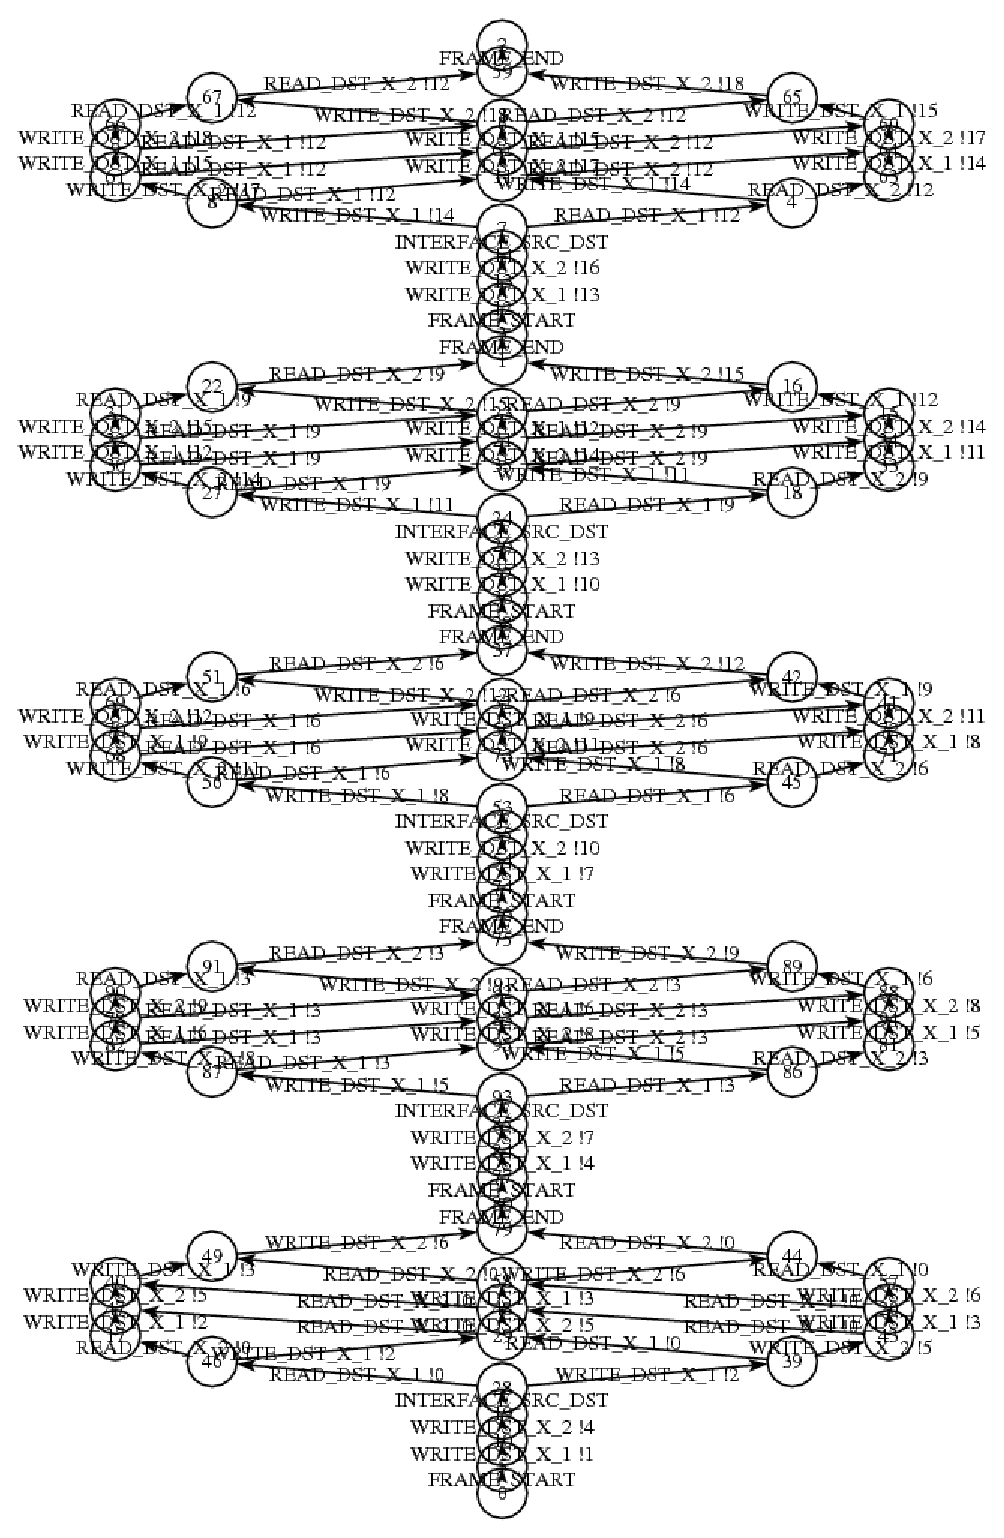
\includegraphics[scale=0.75]{figs/second_order}
\caption{The LTS of the $2^{nd}$ order filter system}
\label{fig:second_order}
\end{figure}

\newpage
\section{Conclusion and future work}
This chapter considered a fundamental issue of real-time control
systems, that of deterministic data flow between different units of
the system. The resolution of this problem---which is very simple in a
synchronous setting---necessitates an involved solution to resolve
properly if the runtime is process-based, i.e., asynchronous. A method
of modeling the deterministic communication construct in AADL via the
use of a new property was presented. The ARC code generator was also
modified to enable generation of Ada code that is Ravenscar-compliant,
creating specialized connectors based on the exchanger protected
object pattern that ensures this protocol. The solution is elegant in
that it does not increase the thread population of the system and does
not involve any impact from the communication code to the functional
code and vice versa.

The DBX connectors and their implementation are a necessary step
towards the acceptance of the AADL language as a viable tool for
control system design. With these connectors, code generated from AADL
models to run on Ravenscar-compliant kernels provides a clean method
of implementing control systems using an ADL to describe the
architecture of a system. They also alleviate the problem of data
inconsistency in case a thread has more than one incoming data
port. Such a thread may be preempted by the source thread after it has
read one port but before it has read the others. The source thread may
then write a new set of data on the ports causing the thread in
question to read the new data for the unread ports when it
resumes. However, this is irrelevant with DBX as the source thread
writes in a separate part of the buffer compared to the part of the
buffer that the destination thread reads from. Another advantage is
that the communication code is completely separate and orthogonal to
the functional code, which is within the thread callbacks. This
eliminates undue coupling within modules that can lead to difficulty
in maintainability.

The particular instance of the provided solution---architecture in
AADL and source code in Ada---is specific to the Ravenscar Profile and
its semantics. However, this approach, in general, would be applicable
to hard real-time systems running on a process-based executive as
well, provided the system hypotheses as enunciated are fulfilled by
the operating system. These hypotheses include rate monotonic or
deadline monotonic priority assignment, a fixed-priority preemptive
scheduler, the priority ceiling protocol for mutexes and synchronous
release for threads that become ready at the same time.

Also provided were details of the automatically generated LOTOS code
that provides verification capability by modeling the data flow aspect
of the system. There exists justification for the use of such
verification artifacts \emph{in lieu} of exhaustive test cases to
achieve certification, specifically for flight software.

Since actual control systems might be based upon algorithms that
involve calculations based not only on the immediately preceding
values, but those from even earlier samples, therefore, a higher-order
deterministic form of the DBX connectors was also developed. These
connectors can be used to provide buffering logic that is
automatically generated and can be used to rapidly code these control
laws. The addition of the \texttt{Hyperperiod\_Age} property to AADL
allows modeling these higher-order connectors, and ARC generates
correctly dimensioned higher-order stepper or stagger DBX connectors
to handle the data flow between threads. ARC also generates LOTOS code
for the automatic verification of these higher-order connectors.

Future work on this axis of research includes mainly the
implementation of AADL ``modes''. AADL modes allow for different
system configurations of a component at runtime that can be changed as
a function of the events received by it over its \texttt{in event port}
or \texttt{in out event port} features. A component can change
property associations per mode, it can enable or disable internal
connections, or even activate or deactivate its contained threads (in
case of a process implementation). This allows the expression in the
model of large-grain behavior of the system. Implementing modes in
a code generator like ARC is a proposition with varied complexity
according to what is to be supported.

The most basic mode-dependent behavior is that of changing the
\texttt{Compute\_Entrypoint} property of a thread with a mode
change. This could be implemented via a modification of the generated
dispatch procedures. In case of an event reception that changes to a
mode that stipulates another entrypoint, a global variable could be
changed to reflect that, this variable would then be consulted by the
dispatch procedure and it would decide which entrypoint to call based
on its value.

Similarly, enabling and disabling of connections is quite simple to
implement. A global variable that stores the current mode can be
checked in the API procedures that are generated in each functional
unit package to access the exchangers and synchronizers. If the
corresponding connection is enabled, the generated procedure writes to
the concerned exchanger or synchronizer, otherwise it doesn't and
returns.

Mode changes that involve a modification of the \texttt{Period} or
\texttt{Deadline} properties of threads, however, are not so
simple. This is so because a change in either of these properties may
move a thread's base priority higher or lower if it passes through
that of another thread. Since task base priorities in Ada Ravenscar
are static and cannot be changed at runtime, this would break the
schedulability analysis. However, in~\cite{puente@adalett01}, the
authors have proposed a novel technique to achieve just that. The
solution proposes to decouple the Ada task construct from the
\emph{jobs} of the tasks. A task may call the callback code of one or
another conceptual functionality (job) depending on the required
priority of the conceptual functionality. In this case, e.g., if there
are two design level threads A and B, with A at a higher priority,
then there would be two Ada tasks generated, named lets say
Task\_One---at higher priority---and Task\_Two. In the nominal case,
Task\_One would call the response code of the design level thread A,
and Task\_Two would invoke code for B. However, if a mode change
occurs that changes design level thread configuration such that thread
B is now at a higher-priority, then Task\_One would call the response
code for thread B, and Task\_Two would invoke the code for A. This
effectively changes the priority of the callbacks, thus meeting design
specifications; \emph{and} it conforms to the static priority
constraint of the Ada Ravenscar Profile because the priorities of the
\emph{tasks} don't change.

The work presented in this chapter has been published in the
\emph{13$^{th}$ IEEE International Conference on Embedded and
  Real-Time Computing Systems and Applications---RTCSA'07}.

%%% Local Variables:
%%% mode: latex
%%% mode: flyspell
%%% TeX-master: t
%%% End:

%%  LocalWords:  preemptions
